\documentclass[13pt,onlymath]{beamer}
\usefonttheme{serif}
\usepackage{graphicx,amsmath,amssymb,tikz,psfrag,epstopdf,fancyvrb}
\usepackage[lighttt]{lmodern}
%\usepackage{graphicx,psfrag}

\input defs.tex

%% formatting

\mode<presentation>
{
\usetheme{default}
}
\setbeamertemplate{navigation symbols}{}
\usecolortheme[rgb={0.13,0.28,0.59}]{structure}
\setbeamertemplate{itemize subitem}{--}
\setbeamertemplate{frametitle} {
    \begin{center}
      {\large\bf \insertframetitle}
    \end{center}
}

\newcommand\footlineon{
  \setbeamertemplate{footline} {
    \begin{beamercolorbox}[ht=2.5ex,dp=1.125ex,leftskip=.8cm,rightskip=.6cm]{structure}
      \footnotesize \insertsection
      \hfill
      {\insertframenumber}
    \end{beamercolorbox}
    \vskip 0.45cm
  }
}
\footlineon

\AtBeginSection[] 
{ 
    \begin{frame}<beamer> 
        \frametitle{Outline} 
        \tableofcontents[currentsection,currentsubsection] 
    \end{frame} 
} 

%% begin presentation

\title{\large \bfseries Basic Graph Algorithms}

\author{Jaehyun Park\\[3ex]
CS 97SI\\
Stanford University}

\date{\today}

\begin{document}

\frame{
\thispagestyle{empty}
\titlepage
}

\section{Graphs}

\begin{frame}{Graphs}
\BIT
\item An abstract way of representing connectivity using nodes (also called vertices) and edges
\item We will label the nodes from $1$ to $n$
\item $m$ edges connect some pairs of nodes
\BIT
\item Edges can be either one-directional (directed) or bidirectional
\EIT
\item Nodes and edges can have some auxiliary information
\EIT
\vfill
\begin{center}
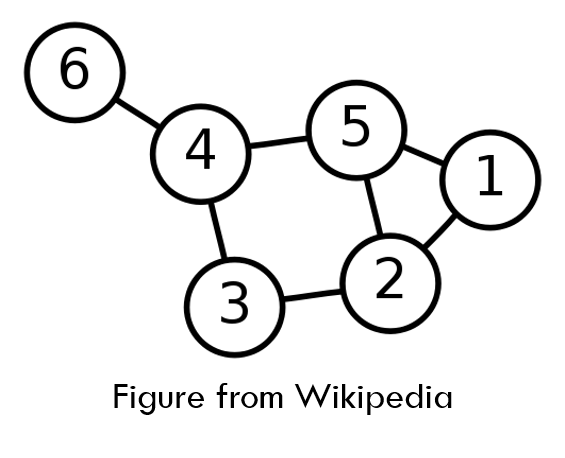
\includegraphics[height=0.3\textheight]{figures/graph_example}
\end{center}
\end{frame}

\begin{frame}{Why Study Graphs?}
\BIT
\item Lots of problems formulated and solved in terms of graphs
\BIT
\item Shortest path problems
\item Network flow problems
\item Matching problems
\item 2-SAT problem
\item Graph coloring problem
\item Traveling Salesman Problem (TSP): \emph{still unsolved!}
\item and many more...
\EIT
\EIT
\end{frame}

\section{Adjacency Matrix and Adjacency List}

\begin{frame}{Storing Graphs}
\BIT
\item Need to store both the set of nodes $V$ and the set of edges $E$
\BIT
\item Nodes can be stored in an array
\item Edges must be stored in some other way
\EIT
\item Want to support operations such as:
\BIT
\item Retrieving all edges incident to a particular node
\item Testing if given two nodes are directly connected
\EIT
\item Use either adjacency matrix or adjacency list to store the edges
\EIT
\end{frame}

\begin{frame}{Adjacency Matrix}
\BIT
\item An easy way to store connectivity information
\BIT
\item Checking if two nodes are directly connected: $O(1)$ time
\EIT
\item Make an $n \times n$ matrix $A$
\BIT
\item $a_{ij} = 1$ if there is an edge from $i$ to $j$
\item $a_{ij} = 0$ otherwise
\EIT
\item Uses $\Theta(n^2)$ memory
\BIT
\item Only use when $n$ is less than a few thousands,
\item \emph{and} when the graph is dense
\EIT
\EIT
\end{frame}

\begin{frame}{Adjacency List}
\BIT
\item Each node has a list of outgoing edges from it
\BIT
\item Easy to iterate over edges incident to a certain node
\item The lists have variable lengths
\item Space usage: $\Theta(n+m)$
\EIT
\EIT
\vfill
\begin{center}
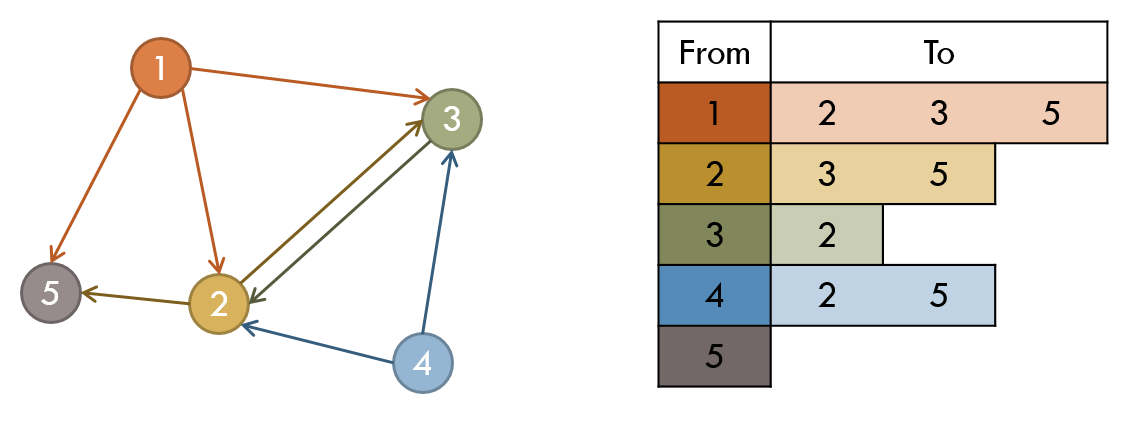
\includegraphics[height=0.4\textheight]{figures/adjlist1}
\end{center}
\end{frame}

\begin{frame}[fragile]{Implementing Adjacency List}
\BIT
\item Solution 1. Using linked lists
\BIT
\item Too much memory/time overhead
\item Using dynamic allocated memory or pointers is bad
\EIT
\item Solution 2. Using an array of \verb.vector.s
\BIT
\item Easier to code, no bad memory issues
\item But very slow
\EIT
\item Solution 3. Using arrays (!)
\BIT
\item Assuming the total number of edges is known
\item Very fast and memory-efficient
\EIT
\EIT
\end{frame}

\begin{frame}{Implementation Using Arrays}
\begin{center}
\includegraphics[height=0.7\textheight]{figures/adjlist2}
\end{center}
\end{frame}

\begin{frame}[fragile]{Implementation Using Arrays}
\BIT
\item Have two arrays \verb,E, of size $m$ and \verb,LE, of size $n$
\BIT
\item \verb,E, contains the edges
\item \verb,LE, contains the starting pointers of the edge lists
\EIT
\item Initialize \verb,LE[i] = -1, for all \verb,i,
\BIT
\item \verb,LE[i] = 0, is also fine if the arrays are 1-indexed
\EIT
\item Inserting a new edge from \verb,u, to \verb,v, with ID \verb,k,
\begin{Verbatim}[xleftmargin=15pt]
E[k].to = v
E[k].nextID = LE[u]
LE[u] = k
\end{Verbatim}
\EIT
\end{frame}

\begin{frame}[fragile]{Implementation Using Arrays}
\BIT
\item Iterating over all edges starting at u:
\begin{Verbatim}[xleftmargin=15pt]
for(ID = LE[u]; ID != -1; ID = E[ID].nextID)
  // E[ID] is an edge starting from u
\end{Verbatim}
\vfill
\item Once built, it's hard to modify the edges
\BIT
\item The graph better be static!
\item But adding more edges is easy
\EIT
\EIT
\end{frame}

\section{Special Graphs}
\begin{frame}{Tree}
\BIT
\item A connected acyclic graph
\item Most important type of special graphs
\BIT
\item Many problems are easier to solve on trees
\EIT
\item Alternate equivalent definitions:
\BIT
\item A connected graph with $n-1$ edges
\item An acyclic graph with $n-1$ edges
\item There is exactly one path between every pair of nodes
\item An acyclic graph but adding any edge results in a cycle
\item A connected graph but removing any edge disconnects it
\EIT
\EIT
\end{frame}

\begin{frame}{Other Special Graphs}
\BIT
\item Directed Acyclic Graph (DAG): the name says what it is
\BIT
\item Equivalent to a partial ordering of nodes
\EIT
\vfill
\item Bipartite Graph: Nodes can be separated into two groups $S$ and $T$ such that edges exist between $S$ and $T$ only (no edges within $S$ or within $T$)
\EIT
\end{frame}

\section{Depth-First and Breadth-First Search}

\begin{frame}{Graph Traversal}
\BIT
\item The most basic graph algorithm that visits nodes of a graph in certain order
\item Used as a subroutine in many other algorithms
\vfill
\item We will cover two algorithms
\BIT
\item Depth-First Search (DFS): uses recursion (stack)
\item Breadth-First Search (BFS): uses queue
\EIT
\EIT
\end{frame}

\begin{frame}{Depth-First Search}
DFS($v$): visits all the nodes reachable from $v$ in depth-first order
\BIT
\item Mark $v$ as visited
\item For each edge $v \rightarrow u$:
\BIT
\item If $u$ is not visited, call DFS($u$)
\EIT
\vfill
\item Use non-recursive version if recursion depth is too big (over a few thousands)
\BIT
\item Replace recursive calls with a stack
\EIT
\EIT
\end{frame}

\begin{frame}{Breadth-First Search}
BFS($v$): visits all the nodes reachable from $v$ in breadth-first order
\BIT
\item Initialize a queue $Q$
\item Mark $v$ as visited and push it to $Q$
\item While $Q$ is not empty:
\BIT
\item Take the front element of $Q$ and call it $w$
\item For each edge $w \rightarrow u$:
\BIT
\item If $u$ is not visited, mark it as visited and push it to $Q$
\EIT
\EIT
\EIT
\end{frame}


\section{Topological Sort}

\begin{frame}{Topological Sort}
\BIT
\item Input: a DAG $G = (V, E)$
\item Output: an ordering of nodes such that for each edge $u \rightarrow v$, $u$ comes before $v$
\item There can be many answers
\BIT
\item \eg, both $\{6, 1, 3, 2, 7, 4, 5, 8\}$ and $\{1, 6, 2, 3, 4, 5, 7, 8\}$ are valid orderings for the graph below
\EIT
\EIT
\begin{center}
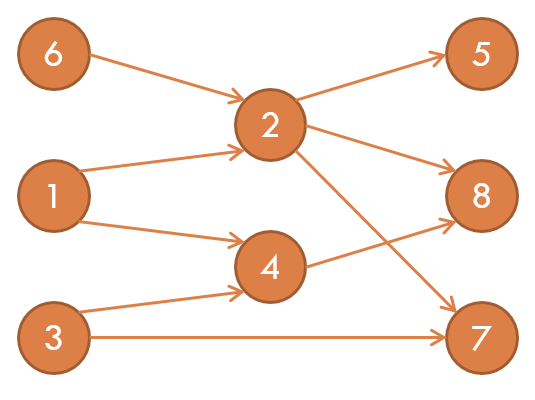
\includegraphics[height=0.3\textheight]{figures/toposort}
\end{center}
\end{frame}

\begin{frame}{Topological Sort}
\BIT
\item Any node without an incoming edge can be the first element
\item After deciding the first node, remove outgoing edges from it
\item Repeat!
\vfill
\item Time complexity: $O(n^2 + m)$
\BIT
\item Too slow...
\EIT
\EIT
\end{frame}

\begin{frame}{Topological Sort (faster version)}
\BIT
\item Precompute the number of incoming edges $\mathrm{deg}(v)$ for each node $v$
\item Put all nodes $v$ with $\mathrm{deg}(v) = 0$ into a queue $Q$
\item Repeat until $Q$ becomes empty:
\BIT
\item Take $v$ from $Q$
\item For each edge $v \rightarrow u$:
\BIT
\item Decrement $\mathrm{deg}(u)$ (essentially removing the edge $v\rightarrow u$)
\item If $\mathrm{deg}(u) = 0$, push $u$ to $Q$
\EIT
\EIT
\item Time complexity: $\Theta(n+m)$
\EIT
\end{frame}


\section{Eulerian Circuit}

\begin{frame}{Eulerian Circuit}
\BIT
\item Given an undirected graph $G$
\item Want to find a sequence of nodes that visits every edge exactly once and comes back to the starting point
\vfill
\item Eulerian circuits exist if and only if
\BIT
\item $G$ is connected
\item \emph{and} each node has an even degree
\EIT
\EIT
\end{frame}

\begin{frame}{Constructive Proof of Existence}
\BIT
\item Pick any node in $G$ and walk randomly without using the same edge more than once
\item Each node is of even degree, so when you enter a node, there will be an unused edge you exit through
\BIT
\item Except at the starting point, at which you can get stuck
\EIT
\item When you get stuck, what you have is a cycle
\BIT
\item Remove the cycle and repeat the process in each connected component
\item Glue the cycles together to finish!
\EIT
\EIT
\end{frame}


\begin{frame}{Related Problems}
\BIT
\item Eulerian path: exists if and only if the graph is connected and the number of nodes with odd degree is $0$ or $2$.
\vfill
\item Hamiltonian path/cycle: a path/cycle that visits every \emph{node} in the graph exactly once. Looks similar but very hard (still unsolved)!
\EIT
\end{frame}


\section{Minimum Spanning Tree (MST)}

\begin{frame}{Minimum Spanning Tree (MST)}
\BIT
\item Given an undirected weighted graph $G = (V, E)$
\item Want to find a subset of $E$ with the minimum total weight that connects all the nodes into a tree
\vfill
\item We will cover two algorithms:
\BIT
\item Kruskal's algorithm
\item Prim's algorithm
\EIT
\EIT
\end{frame}

\begin{frame}{Kruskal's Algorithm}
\BIT
\item Main idea: the edge $e^\star$ with the smallest weight has to be in the MST
\item Simple proof:
\BIT
\item Assume not. Take the MST $T$ that doesn't contain $e^\star$.
\item Add $e^\star$ to $T$, which results in a cycle.
\item Remove the edge with the highest weight from the cycle.
\BIT
\item The removed edge cannot be $e^\star$ since it has the smallest weight.
\EIT
\item Now we have a better spanning tree than $T$
\item Contradiction!
\EIT
\EIT
\end{frame}

\begin{frame}{Kruskal's Algorithm}
\BIT
\item Another main idea: after an edge is chosen, the two nodes at the ends can be merged and considered as a single node (supernode)
\item Pseudocode:
\BIT
\item Sort the edges in increasing order of weight
\item Repeat until there is one supernode left:
\BIT
\item Take the minimum weight edge $e^\star$
\item If $e^\star$ connects two different supernodes, then connect them and merge the supernodes (use union-find)
\EIT
\item Otherwise, ignore $e^\star$ and try the next edge
\EIT
\EIT
\end{frame}

\begin{frame}{Prim's Algorithm}
\BIT
\item Main idea:
\BIT
\item Maintain a set $S$ that starts out with a single node $s$
\item Find the smallest weighted edge $e^\star = (u, v)$ that connects $u \in S$ and $v \notin S$
\item Add $e^\star$ to the MST, add $v$ to $S$
\item Repeat until $S = V$
\EIT
\vfill
\item Differs from Kruskal's in that we grow a single supernode $S$ instead of growing multiple ones at the same time
\EIT
\end{frame}

\begin{frame}{Prim's Algorithm Pseudocode}
\BIT
\item Initialize $S := \{s\}$, $D_v := \mathrm{cost}(s, v)$ for every $v$
\BIT
\item If there is no edge between $s$ and $v$, $\mathrm{cost}(s, v) = \infty$
\EIT
\item Repeat until $S = V$:
\BIT
\item Find $v \notin S$ with smallest $D_v$
\BIT
\item Use a priority queue or a simple linear search
\EIT
\item Add $v$ to $S$, add $D_v$ to the total weight of the MST
\item For each edge $(v, w)$:
\BIT
\item Update $D_w := \min(D_w, \mathrm{cost}(v, w))$
\EIT
\EIT
\item Can be modified to compute the actual MST along with the total weight
\EIT
\end{frame}

\begin{frame}{Kruskal's vs Prim's}
\BIT
\item Kruskal's Algorithm
\BIT
\item Takes $O(m \log m)$ time
\item Pretty easy to code
\item Generally slower than Prim's
\EIT
\item Prim's Algorithm
\BIT
\item Time complexity depends on the implementation:
\BIT
\item Can be $O(n^2+m)$, $O(m \log n)$, or $O(m + n \log n)$
\EIT
\item A bit trickier to code
\item Generally faster than Kruskal's
\EIT
\EIT
\end{frame}


\section{Strongly Connected Components (SCC)}

\begin{frame}{Strongly Connected Components (SCC)}
\BIT
\item Given a \emph{directed} graph $G = (V, E)$
\item A graph is \emph{strongly connected} if all nodes are reachable from every single node in $V$
\item Strongly connected components of $G$ are maximal strongly connected subgraphs of $G$
\item The graph below has 3 SCCs: $\{a, b, e\}$, $\{c, d, h\}$, $\{f, g\}$
\EIT
\begin{center}
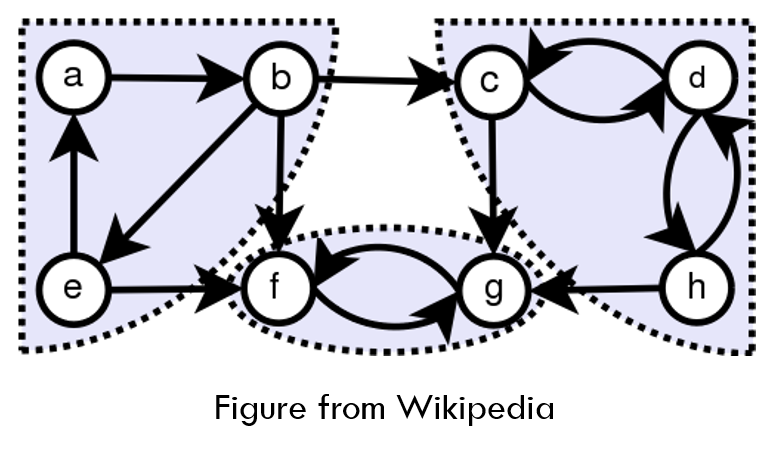
\includegraphics[height=0.3\textheight]{figures/scc_example}
\end{center}
\end{frame}

\begin{frame}{Kosaraju's Algorithm}
\BIT
\item Initialize counter $c := 0$
\item While not all nodes are labeled:
\BIT
\item Choose an arbitrary unlabeled node $v$
\item Start DFS from $v$
\BIT
\item Check the current node $x$ as visited
\item Recurse on all unvisited neighbors
\item After the DFS calls are finished, increment $c$ and set the label of $x$ as $c$
\EIT
\EIT
\item Reverse the direction of all the edges
\item For node $v$ with label $n, n-1, \ldots, 1$:
\BIT
\item Find all reachable nodes from $v$ and group them as an SCC
\EIT
\EIT
\end{frame}

\begin{frame}{Kosaraju's Algorithm}
\BIT
\item We won't prove why this works
\item Two graph traversals are performed
\BIT
\item Running time: $\Theta(n+m)$
\EIT
\vfill
\item Other SCC algorithms exist but this one is particularly easy to code
\BIT
\item and asymptotically optimal
\EIT
\EIT
\end{frame}

\end{document}
